\documentclass[xcolor=table]{beamer}
\usepackage{beamerthemeCambridgeUS}
\usepackage{color}  % for \textcolor{red}{blah}
\usepackage{graphicx}
\usepackage{subfigure}
\usepackage{multicol}
\usepackage{verbatim} % for \begin{comment}
\usepackage{lipsum}


\newcommand\Fontvi{\fontsize{6}{7.2}\selectfont}


\newenvironment{packed_enum}{
\begin{enumerate}
  \setlength{\itemsep}{1pt}
  \setlength{\parskip}{0pt}
  \setlength{\parsep}{0pt}
}{\end{enumerate}}

\newenvironment{packed_item}{
\begin{itemize}
  \setlength{\itemsep}{1pt}
  \setlength{\parskip}{0pt}
  \setlength{\parsep}{0pt}
}{\end{itemize}}

\usetheme{CambridgeUS}

\title{Discrete Mathematics}
\author[Geoffrey Buhl]{Geoffrey Buhl \\ \texttt{geoffrey.buhl@csuci.edu}}
\institute[CSUCI]{California State University Channel Islands}
\date{week 8 class 1}

\def \vec{{\rm vec}}
\newtheorem{conjecture}[theorem]{Conjecture}
\newtheorem{explanation}[theorem]{Explanation}


\begin{document}

%\frame{\titlepage}

%\section[Outline]{}
%\frame{\tableofcontents}

\section{Week 7 Class 1}


\frame
{
  \frametitle{Non-linear Recurrences}

We explore some of the complexities of non-linear recurrences and solve one example of a non-linear recurrence for the Catalan numbers.

\vfill
Class Session Goals:
\begin{packed_enum}
\item Become familar with multiple examples of the Catalan numbers.
\item Demonstrate using the generating function method to solve non-linear recurrence relations.
\end{packed_enum}
\vfill
}

\frame
{
  \frametitle{One homework exercise from last week}

Find the first 5 terms of the Taylor expansion at $x=0$ of $\sqrt{1-4x}$.  By examining the pattern of coefficients find $a_n$ where $\sqrt{1-4x}=\sum_{n=0}^{\infty}a_nx^n$.\vfill

\underline{Answer}\\
$\sqrt{1-4x}=1-2 x-2 x^2-4 x^3-10 x^4-28 x^5+\cdots$\\
or\\
$\sqrt{1-4x}=1-\frac{1}{2^1 1!}4^1x-\frac{1\cdot 3}{2^2 2!}4^2 x^2-\frac{1\cdot 3 \cdot 5}{2^3 3!}4^3 x^3-\frac{1\cdot 3 \cdot 5 \cdot 7}{2^4 4!}4^4 x^4-\frac{1\cdot 3 \cdot 5 \cdot 7 \cdot 9}{2^5 5!}4^5 x^5+\cdots$
}

\frame
{
  \frametitle{Another homework exercise from last week}


Prove $$\frac{1\cdot 3 \cdot 5 \cdots (2n-1)}{2^n (n+1)!}4^n=\frac{1}{n+1} \binom{2n}{n}.$$


}



\frame
{
  \frametitle{Catalan Numbers Activity}

In small groups, work on the ``Catalan Numbers'' worksheet. The goals of this worksheet are to:
\vfill
\begin{packed_enum}
\item Find some initial values of the Catalan number.
\item Begin to explore the recursive formula for the Catalan numbers
\end{packed_enum}
\pause
\vfill
%\underline{Catalan numbers}\\ 1, 1, 2, 5, 14, 42, 132, 429, $\ldots$ (A000108)
%\pause


}

\frame
{
  \frametitle{Catalan Numbers Activity}

  \begin{figure}[htp]
  \begin{center}
    \subfigure{
\includegraphics[scale=.15]{dyck_path_5}}
    \end{center}
\end{figure}


}

\frame
{
  \frametitle{Catalan Numbers Activity}

In small groups, work on the ``Catalan Numbers'' worksheet. The goals of this worksheet are to:
\vfill
\begin{packed_enum}
\item Find some initial values of the Catalan number.
\item Begin to explore the recursive formula for the Catalan numbers
\end{packed_enum}
\pause
\vfill
\underline{Catalan numbers}\\ 1, 1, 2, 5, 14, 42, 132, 429, $\ldots$ (A000108)


}

\frame
{
  \frametitle{Create the Catalan Numbers Recurrence (n=6 case)}

  \begin{figure}[htp]
  \begin{center}
    \subfigure{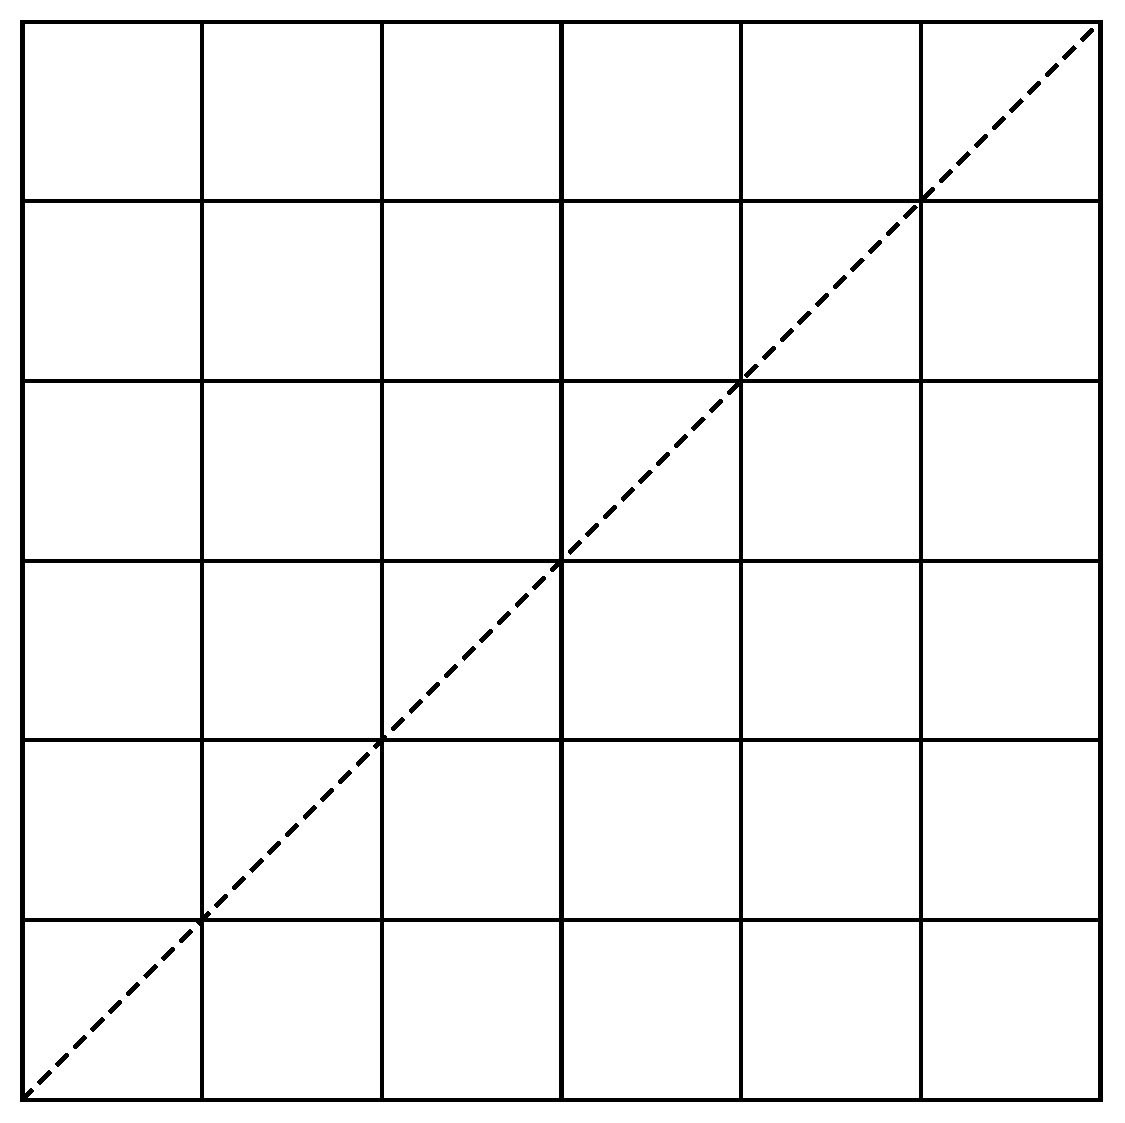
\includegraphics[scale=.35]{catalan_grid}}
    \end{center}
\end{figure}

}

\frame
{
  \frametitle{Catalan Numbers Recurrence}

For $n=6$, $C_6=C_0C_5+C_1c_4+C_2C_3+C_3C_2+C_4C_1+C_5C_0$ and in general we have

$C_n=C_0C_{n-1}+C_1C_{n-2}+C_2C_{n-3}+ \cdots+C_{n-1}C_0$ or

$C_n=\sum_{i=0}^{n-1} C_iC_{n-1-i}$
}





\frame
{
  \frametitle{Closed form solution via the Generating Function method}

Catalan numbers recurrence:\\
$C_n=\sum^{n-1}_0 C_i \cdot C_n-1-i$ with $C_0=1$.\vfill

$C_1=C_0\cdot C_0$\\
$C_2=C_0\cdot C_1+C_1\cdot C_0$\\
$C_3=C_0\cdot C_2+C_1\cdot C_1+C_2\cdot C_0$\\
$C_4=C_0\cdot C_3+C_1\cdot C_2+C_2\cdot C_1+C_3\cdot C_0$\\
$C_5=C_0\cdot C_4+C_1\cdot C_3+C_2\cdot C_2+C_3\cdot C_1+C_4\cdot C_0$\\

\vfill
Let $f(x)=\sum^\infty_0 C_nx^n$ .... So let's try $f(x)^2$.

}


\frame
{
  \frametitle{Use Generating function}

\begin{flalign}
f(x)^2 =&(C_0+C_1x+C_2x^2+C_3x^3+C_4x^4+C_5x^5+\cdots)\\
\cdot&(C_0+C_1x+C_2x^2+C_3x^3+C_4x^4+C_5x^5+\cdots)
\end{flalign}

\vfill
So $f(x)^2=$
\begin{center}
\begin{tabular}{ c c c c c c c }
 \cellcolor{blue!0}$C_0C_0+$ & \cellcolor{green!0}$C_0C_1x+$ & \cellcolor{orange!0}$C_0C_2x^2+$ & \cellcolor{brown!0}$C_0C_3x^3+$ & \cellcolor{black!0}$C_0C_4x^4+$ & $C_0C_5x^5+$ & $\cdots$ \\ 
\cellcolor{green!0}$C_1C_0x+$ & \cellcolor{orange!0}$C_1C_1x^2+$ &\cellcolor{brown!0} $C_1C_2x^3+$ & \cellcolor{black!0}$C_1C_3x^4+$ & $C_1C_4x^5+$ & $C_1C_5x^6+$ & $\cdots$ \\ 
\cellcolor{orange!0}$C_2C_0x^2+$ & \cellcolor{brown!0}$C_2C_1x^3+$ & \cellcolor{black!0}$C_2C_2x^4+$ & $C_2C_3x^5+$ & $C_2C_4x^6+$ & $C_2C_5x^7+$ & $\cdots$ \\  
\cellcolor{brown!0}$C_3C_0x^3+$ & \cellcolor{black!0}$C_3C_1x^4+$ & $C_3C_2x^5+$ & $C_3C_3x^6+$ & $C_3C_4x^7+$ & $C_3C_5x^8+$ & $\cdots$ \\ 
\cellcolor{black!0}$C_4C_0x^4+$ & $C_4C_1x^5+$ & $C_4C_2x^6+$ & $C_4C_3x^7+$ & $C_4C_4x^8+$ & $C_4C_5x^9+$ & $\cdots$ \\
$\vdots$ & $\vdots$ & $\vdots$ & $\vdots$ & $\vdots$ & $\vdots$ & $\ddots$
\end{tabular}
\end{center}
\vfill


}


\frame
{
  \frametitle{Use Generating function}

\vfill
So $f(x)^2=$
\begin{center}
\begin{tabular}{ c c c c c c c }
 \cellcolor{blue!15}$C_0C_0+$ & \cellcolor{green!15}$C_0C_1x+$ & \cellcolor{orange!15}$C_0C_2x^2+$ & \cellcolor{brown!15}$C_0C_3x^3+$ & \cellcolor{black!10}$C_0C_4x^4+$ & $C_0C_5x^5+$ & $\cdots$ \\ 
\cellcolor{green!15}$C_1C_0x+$ & \cellcolor{orange!15}$C_1C_1x^2+$ &\cellcolor{brown!15} $C_1C_2x^3+$ & \cellcolor{black!10}$C_1C_3x^4+$ & $C_1C_4x^5+$ & $C_1C_5x^6+$ & $\cdots$ \\ 
\cellcolor{orange!15}$C_2C_0x^2+$ & \cellcolor{brown!15}$C_2C_1x^3+$ & \cellcolor{black!10}$C_2C_2x^4+$ & $C_2C_3x^5+$ & $C_2C_4x^6+$ & $C_2C_5x^7+$ & $\cdots$ \\  
\cellcolor{brown!15}$C_3C_0x^3+$ & \cellcolor{black!10}$C_3C_1x^4+$ & $C_3C_2x^5+$ & $C_3C_3x^6+$ & $C_3C_4x^7+$ & $C_3C_5x^8+$ & $\cdots$ \\ 
\cellcolor{black!10}$C_4C_0x^4+$ & $C_4C_1x^5+$ & $C_4C_2x^6+$ & $C_4C_3x^7+$ & $C_4C_4x^8+$ & $C_4C_5x^9+$ & $\cdots$ \\
$\vdots$ & $\vdots$ & $\vdots$ & $\vdots$ & $\vdots$ & $\vdots$ & $\ddots$
\end{tabular}
\end{center}
\vfill
\pause
$=\textcolor{blue}{C_1}+\textcolor{green}{C_2}x+\textcolor{orange}{C_3}x^2+\textcolor{brown}{C_4}x^3+C_5x^4 + \cdots$

}


\frame
{
  \frametitle{Use Generating function}

$f(x)^2=xf(x)-1$

}

\frame
{
  \frametitle{Taylor Series}

$f(x)^2=xf(x)-1$

}

\frame
{
  \frametitle{Final Formula}

$f(x)^2=xf(x)-1$

}

\frame
{
  \frametitle{Create the Catalan Numbers Recurrence (n=6 case)}

  \begin{figure}[htp]
  \begin{center}
    \subfigure{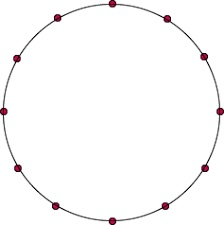
\includegraphics[scale=.9]{12table}}
    \end{center}
\end{figure}

}

\frame
{
  \frametitle{Closed form solution via the Generating Function method}

Catalan numbers recurrence:\\
$C_n=\sum^{n-1}_0 C_i \cdot C_n-1-i$ with $C_0=1$.\vfill

$C_1=C_0\cdot C_0$\\
$C_2=C_0\cdot C_1+C_1\cdot C_0$\\
$C_3=C_0\cdot C_2+C_1\cdot C_1+C_2\cdot C_0$\\
$C_4=C_0\cdot C_3+C_1\cdot C_2+C_2\cdot C_1+C_3\cdot C_0$\\
$C_5=C_0\cdot C_4+C_1\cdot C_3+C_2\cdot C_2+C_3\cdot C_1+C_4\cdot C_0$\\

\vfill
Let $f(x)=\sum^\infty_0 C_nx^n$ .... So let's try $f(x)^2$.

}





\frame
{
  \frametitle{Frogs and Toads Puzzle}

 Below is the $n=3$ version of the puzzle.
\begin{figure}[htp]
  \begin{center}
    \subfigure{
\includegraphics[scale=.65]{frogs}}
  \end{center}
\end{figure}

Let $m_n$ be the minimum number of moves (jumps or slides) in a winning strategy.  Can you express $m_n$ as a recurrence relation?  What's it's generating function?  Can you find a closed form solution?

}



\frame
{
  \frametitle{Non-Homogenous Linear}

What are the recurrence relations, generating functions, and closed for solutions for $c_n$, $T_n$, and $a_n$?

Sequence 1: $1,1,1,1, \cdots$, $b_n=b_{n-1}$, $b_0=1$\\
Sequence 2: $1,2,3,4, \cdots$, $c_n=\sum_{i=0}^n b_i$\\
Sequence 3: $1,3,6,10, \cdots$, $T_n=\sum_{i=0}^n c_i$\\
Sequence 4: $1,4,10,20, \cdots$, $a_n=\sum_{i=0}^n T_i$\\
$\vdots$ \\
Sequence n: ???

What is sequence n? recurrence? generating function? closed form?

}






\frame
{
  \frametitle{From the homework/class}

Ternary strings with double zeros.

\vfill
or
\vfill


Runs of 1s in binary strings
}

\end{comment}


\end{document}

